\documentclass{article}
\usepackage[utf8]{inputenc}
\usepackage[spanish]{babel}
\usepackage[pdftex]{graphicx}
\usepackage{listings}
\usepackage{parskip}
\usepackage{fancyhdr}
\usepackage{amsmath}
\usepackage{indentfirst}
\usepackage{vmargin}
\setmarginsrb{3 cm }{ 2.5cm }{3 cm }{2.5 cm}{1 cm}{1.5 cm}{1 cm}{1.5 cm}
\title{Binarytree}
\author{Martin, Francisco Manuel \\
        Martinez, Victor
}

\makeatletter
\let\thetitle\@title
\let\theauthor\@author
\let\thedate\@date
\makeatother
\pagestyle{fancy}
\fancyhf{}
\rhead{\theauthor}
\lhead{\thetitle}
\cfoot{\thepage}
%\addto\captionspanish{
\renewcommand*\contentsname{Índex}%}
\setlength{\parindent}{1cm}

\begin{document}
    \begin{titlepage}
	\centering
    \vspace*{0.5 cm}

    \textsc{\LARGE Universidad Politécnica de Lleida}\\[2.0 cm]	% University Name
	\textsc{\large Practica 5}\\[0.5 cm]				% Course Name
	\rule{\linewidth}{0.2 mm} \\[0.4 cm]
	{ \huge \bfseries \thetitle}\\
	\rule{\linewidth}{0.2 mm} \\[1.5 cm]

	\begin{minipage}{0.4\textwidth}
		\begin{flushleft} \large
			\emph{Author:}\\
			\theauthor
			\end{flushleft}
			\end{minipage}~
			\begin{minipage}{0.4\textwidth}
			\begin{flushright} \large
			\emph{DNI:} \\
			48057095k \\
			78100640T% Your Student Number
		\end{flushright}
	\end{minipage}\\[2 cm]

	{\large \thedate}\\[2 cm]

	\vfill

\end{titlepage}
\tableofcontents
\pagebreak


\section{Tarea 1: Implementación de los árboles binarios}
    \subsection{Constructores}
    En esta sección solo vamos a comentar un pequeño detalle sobre el tercer constructor. \newline
    Tratamos \textbf{left} y \textbf{right} de manera que, si uno de ellos es null inicializamos la instancia de Node correspondiente a null. \newline
    de esta manera,evitamos un NullPointerException en caso de intentar acceder al atributo root del árbol en cuestión.

    \subsection{método equals}
        \subsubsection{equals de LinkedBinaryTree}
            En primer lugar, comprobamos que el objecto de tipo \textit{Object} pasado como parámetro apunte a una instancia de LinkedBinaryTree.
            Si es así, realizamos un cast y ejecutamos el método estático \textit{recEquals} de la clase Node que comprobará recursivamente si los \textit{roots} de los árboles son iguales.
    \subsubsection{equals de Node}
            Aunque este método no lo usamos en LinkedBinaryTree ya que directamente empleamos el método \textit{recEquals}, nunca está de más definir el método equals dentro de una classe.
            En este caso comprobamos que el parámetro \textit{obj} apunte a una instancia de Node y 
            ejecutamos el método \textit{recEquals}
    \subsubsection{método recEquals}
            En primer lugar, comprobamos si alguno de los parámetros apunta a null, si es así devolvemos el resultado de igualar los dos parámetros (si uno es null el otro también debe serlo para cumplir la igualdad).
            En caso contrario seguimos comprobando si los dos nodos son iguales (Contienen el mismo elemento y sus nodos derecho e izquierdo son también iguales).
            \newline
            
\section{Tarea 2: Recorridos iterativos en árboles binarios}

    \subsection{Interfaz Traversals}
    \textbf{ ¿Qué diferencias provocaría que la interfaz fuera genérica y los
        métodos no?}\\
            En caso de que los métodos sean genéricos y la clase no, podremos usar los métodos con cualquier BinaryTree sin importar de que tipo sean los elementos que contiene.
            
            En cambio, si implementamos la interfaz de manera genérica y los métodos no-genericos, solo podremos usar dichos métodos con árboles binarios que contengan elementos del mismo tipo con el cual hemos inicializado la instancia de \textbf{Traversals}, \newline por lo cual necesitaremos crear una instancia de \textbf{Traversals} para cada árbol binario que definamos con un tipo distinto.
            
       \subsection{Clase IterativeTraversals}
            En esta clase implementamos los diferentes recorridos en profundidad sobre árboles binarios de manera iterativa. \newline
            Los stacks con los que trabajamos contendrán elementos de tipo BinaryTree, y así iremos comprobando si están vacíos o no para realizar las operaciones.\newline
            En la explicación de los siguientes métodos voy a referirme algunas
            veces a \textit{el último elemento introducido en el stack} como el elemento que contiene el root del árbol que es el objeto con el que realmente trabajamos.
            
        \subsubsection{Preorder}
        Como debemos recorrer los nodos con el patrón \textit{Parent},
        \textit{left}, \textit{right}, en este algoritmo empezamos añadiendo al stack el árbol introducido como parametro.\newline
        Vamos añadiendo a la lista el último elemento introducido en el stack y llenando el stack con los hijos derecho e izquierdo del elemento, tal y como lo plantearíamos en el algoritmo recursivo.
        
        \subsubsection{Inorder}
        La idea del algoritmo implementado para éste recorrido (\textit{left}, \textit{parent}, \textit{right}) se basa en posicionarse en el elemento más a la izquierda del árbol y, en cuanto lo encontramos lo añadimos a la lista, añadimos a su padre (que estamos seguros de que será el último elemento añadido en el stack) y visitamos el hijo derecho. \newline
        Seguimos hasta que el stack esté vacío y el último árbol visitado esté vacío también.
        
        \subsubsection{Postorder}
        El algoritmo implementado en éste recorrido (\textit{left}, \textit{right}, \textit{parent})
        se basa en una idea un poco diferente a las anteriores.\newline
        Se trata en mirar el recorrido de manera inversa, por lo que recorreremos de \textit{Parent} a \textit{right} a \textit{left} y iremos añadiendo los elementos al principio de la lista y no al final. De esta manera, el código nos queda muy simple y prácticamente igual a la implementación de PreOrder solo que cambiando el orden en que añadimos los hijos.  \newline
        Cabe destacar que es necesario que la lista sea de tipo \textit{LinkedList} para que las inserciones sean óptimas, en caso de ser un \textit{ArrayList} estaríamos aumentando el coste del algoritmo prácticamente de manera exponencial.
        

\section{Tarea 3: Reconstrucción del árbol binario}
La idea en la resolución de éste método se basa en los dos argumentos siguientes:
\begin{enumerate}
    \item El último elemento de la lista que contiene los elementos en postOrden siempre será el root del árbol.
    \item Debemos encontrar la posición de ese elemento en la lista de inOrden para de esta manera, poder separar los elementos que se encuentran a su izquierda y a su derecha como árbol izquierdo y árbol derecho.
\end{enumerate}
Siguiendo estas dos premisas implementamos el método de manera recursiva mediante sublistas.
\begin{centering}
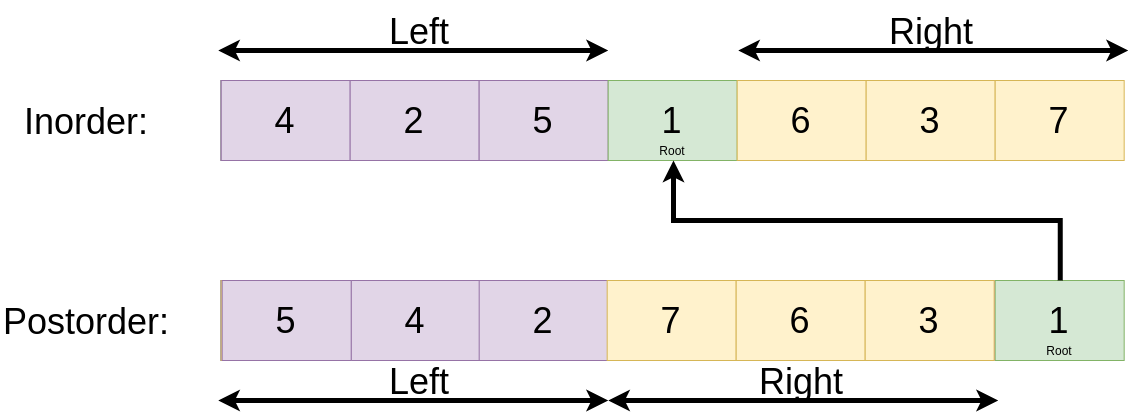
\includegraphics[scale=0.36]{Diagram.png}
\end{centering}
\section{Conclusiones}

Durante la resolución del laboratorio hemos aprendido bastante sobre como trata Java los genéricos en tiempo de compilación (mediante el proceso de \textit{type erasure}).
Como java en tiempo de ejecución no tiene información sobre los tipos genéricos, es un error realizar un cast de la siguiente manera:
\begin{verbatim}
Node<E> node = (Node<E>) obj;
\end{verbatim}
\newline
Y en su lugar debemos utilizar comodines:
\begin{verbatim}
Node<?> node = (Node<?>) obj;
\end{verbatim}
De esta manera,evitamos un posible error de ejecución.

En la implementación del método \textit{postAndIn} estubimos debatiendo sobre si implementarlo utilizando índices o sublistas.\newline
En el primer caso, la idea se basaba en utilizar 4 índices (2 índices indicando el principio y el final del segmento que queríamos tratar sobre la lista postOrder y 2 índices indicando los mismos parámetros sobre la lista inOrder).\newline
En el segundo caso simplemente vamos reduciendo los segmentos a tratar generando sublistas, por lo que nos parecía que era más ineficiente que el primer caso.\newline
En cambio, después de adentrarnos en el codigo fuente de la clase ArrayList vimos que el método sublist no genera una lista nueva, sino que devuelve una vista sobre la lista original, por lo que siempre trabajamos sobre el mismo objeto y de una manera muy parecida al primer caso que hemos comentado en el que trabajamos siempre sobre las mismas listas acotando segmentos mediante índices.\newline
El método sublist de la clase LinkedList (heredado de la clase AbstractList) se
basa en la misma idea, pero el coste de realizar la operación get va a ser
mayor, ya que  cuando lo hagamos sobre una sublista, realmente se va a realizar
sobre la lista original por lo que el coste de realizar dicho get siempre va a
ser O(n).

\end{document}
